\documentclass[11pt]{amsart}
\usepackage[colorlinks=true]{hyperref}
\usepackage{graphicx}
\usepackage{float}
\usepackage{listings}


\title{ScalABM}
\author{David R. Pugh, Daniel F. Tang, J. Doyne Farmer}
\date{\today}

\begin{document}
\maketitle

\section{Objective}
ScalABM is a \textit{community driven}, \textit{open-source} project to develop a \textit{user-friendly} modeling platform and tool stack for building \textit{scalable}, \textit{data-driven}, and \textit{reproducible} agent-based models (ABMs) of \textit{economic} systems on the JVM using \href{http://www.scala-lang.org/}{Scala} and \href{http://akka.io/}{Akka}.

\subsection{General requirements}
The high-level architecture design and the software development processes of the ScalABM project should mimic the layered architecture design and open-source development processes that have become standard ``best practices'' for developing \href{http://www.reactivemanifesto.org/}{Reactive} ``Fast Data'' web applications.\footnote{
%
See figure 1 from \href{./fast-data-big-data-evolved.pdf}{Wampler (2015)} for a similar high-level summary of a Reactive, ``Fast Data'' web application architecture.
%
}
\subsubsection{...community driven, open source...}
Progress in the building of large scale models of economic systems has been significantly hindered by...
\begin{itemize}
    \item ...the lack of a common modeling platform as well as a common tool stack for data management and analytics. The lack of a common modeling platform and tool stack has, to a large degree, made it impossible to compare competing models. 
    \item ...the lack of access to model source code. Lack of access to a model's source code dramatically increases the costs associated with reproducing that model's results and makes it difficult or impossible for other researchers to extend that model in the future.
\end{itemize}

The development of all ScalABM libraries will be driven by the needs of the economics ABM community. All software development will take place in public: from the start of the project all source code for the ScalABM project will be hosted on GitHub under a permissive Apache 2.0 license that allows for free use of the software libraries (even in commercial applications).

\subsubsection{...user-friendly...}
The ability to interactively explore ABMs in near-real time is crucial for developing intuition about the mechanisms driving the key results of these models. In order to facilitate interactive exploration of ABMs built using the ScalABM libraries all models should have two, complementary user interfaces:
\begin{enumerate}
    \item a user-friendly, web-browser based user interface based around the \href{https://www.playframework.com/}{Play web framework}. The GUI should leverage existing, high-quality libraries for real-time data streaming, analysis and visualization.
    \item an intuitive and consistent command line interface (CLI). In addition to facilitating efficient batch processing of model simulations (i.e., parameter sweeps), the CLI should allow for easy replication of any particular model simulation.
\end{enumerate}

In addition to making it easy to interactively explore existing ABMs we want to make sure that the ScalABM libraries are structured in a way that minimizes the amount of development time needed to reconfigure and existing model or build a completely new model. In particular...
\begin{itemize}
    \item ...in order to maximize reuse of code, models built using our toolkit should be composed of mostly existing components. Leveraging mostly existing components reduces development time for a new model to that needed to create a few novel components together with the time needed to wire all the desired model components together.
    \item ...the process of wiring model components together (which includes the specification of all model parameters, agent behavioral strategies, etc), sometimes called dependency injection (DI), should be as simple and transparent as possible. The wiring process should be specified in a single, \textit{human-readable}, model configuration file.
    \item ...the build process (i.e., specification of dependencies, platform specific build options, etc) for a particular model should be completely specified in a single build file.
\end{itemize}

\subsubsection{...scalable...}
Aggregate behavior of many (most?) real-world economic systems fundamentally depends on system size. Put another way, system size is a key parameter for modeling economic systems and in order to accurately model the dynamics of some systems, we may need to build and simulate models that are as close to observed scale as possible. 

Broadly speaking, there are two kinds of solutions to the scaling problem...
\begin{itemize}
    \item ...software solutions: ScalABM leverages the \href{https://en.wikipedia.org/wiki/Actor_model}{Actor model} of concurrency as implemented in the \href{http://akka.io/}{Akka} library to build ABMs that are highly concurrent, distributed, and message-driven.
    \item ...hardware solutions:  because models built using the ScalABM libraries are basically scalable web applications, we are able to leverage the massively multi-core cloud computing platforms that are quickly becoming the dominant form of large-scale computing outside of academia.
\end{itemize}

Existing solutions to the scaling problem either rely on access to university (or national) supercomputing resources or leverage the computing power of GPU clusters but then force researchers to express their ABMs in the restrictive GPU computing environment. We believe that our approach to the scaling problem has several benefits over existing solutions.
\begin{itemize}
    \item Outsourcing of cluster management to third party provider. ABMs built using our framework can be ``containerized'' using technologies such as \href{https://www.docker.com/}{Docker} or \href{https://www.vagrantup.com/}{Vagrant} and then deployed on a third-party cloud computing service provider such as \href{http://aws.amazon.com/}{AWS}, \href{https://cloud.google.com/compute/}{Google Compute Engine}, \href{https://www.heroku.com/}{Heroku}, \href{https://mesosphere.com/}{Mesosphere}, etc. This third party provider then handles all of the intricacies involved with scaling up the model on the cluster to meet our needs.
    \item No longer dependent on access to university or national supercomputers enhances the reproducibility or our research.  The ability to ``containerize'' an ABM built using out framework means that researchers not directly involved in developing a model can still access everything (even down to the operating system) necessary to completely reproduce that model's output. The container can be used to run the model locally on a laptop or sent to a third party provider to scale up via the cloud.
\end{itemize}

\subsubsection{...data-driven...}
We want to build ABMs that can be initialized and validated against real-world data. In order for our ABMs to be data-driven, we need to think carefully about how ScalABM we will manage the flow and storage of data (both model generated data as well as real-world data). There are (at least!) three components to data management: access, analytics, and storage.
\begin{itemize}
    \item Access: A running ABM will generate a large volume of data. Model generated data might be stored, sent to a data analytics engine, or logged out to a file(s). Additionally, data will likely flow in the reverse direction.  In particular, agents in a running ABM may need to read data from a data store (for example, we might wish to initialize economic agents using real-world data).
    \item Analytics: A running ABM is a continuous source of data whose volume is not predetermined. Put another way: ABMs generate \href{http://www.reactive-streams.org/}{reactive data streams}.  Our data analytics components should therefore include tooling for processing and analyzing streaming data. In addition to processing and analyzing streaming data, our data analytics tool stack should include tooling for dealing with ``batch'' or ``mini-batch'' computations. Such batch processing jobs would be performed either relatively infrequently on streaming data or upon completion of a model simulation. The \href{http://spark.apache.org/}{Apache Spark} project is a Scala based project for large-scale data analytics that supports batch, mini-batch and stream processing. 
    \item Storage: Our ABMs should have read/write access to a scalable data store. Additionally, the data analytics components will need a source of input data. In order to avoid simulations being I/O bound, our data store should have extremely fast write access. We should design our tool stack to integrate cleanly with leading NoSQL database architectures such as \href{http://cassandra.apache.org/}{Apache Cassandra} and \href{http://neo4j.com/}{Neo4j}.
\end{itemize}

\subsubsection{...economic...}
ScalABM is not intended to be a general purpose platform for ABM. Rather we want to build a toolkit that is designed to facilitate the construction of agent-based models of economic systems. An economy is populated with many seemingly disparate types of agents (i.e., consumers, producers, financiers, government, some markets, etc). We need to distill the core essence (in terms of data and behaviors) of these different agents into a multi-layered Application Programming Interface (API) defining a generic \textit{economic agent} that can then be specialized to the various types of economic agents needed for any particular model. Our hope is that by doing this we can reduce the effort needed for the parts of agent-based modeling that consume a great deal of software development time.  We also hope that by identifying the key components we can build standard, highly modular interfaces that make it easy to interchange components of models.

\subsubsection{...reproducible...}
The results of many (most?) ABMs are not easily reproducible. Often this is due to some combination of lack of availability of source code, poor documentation, and insufficiently detailed research papers. Reproducibility is further hindered by the lack of use of ``best practices'' for software development.

In order to facilitate the reproducibility of results generated by models built using the ScalABM libraries, the source code for all ScalABM libraries will strive to adhere to the following ``best practices''...
\begin{itemize}
    \item ...be under version control using \href{https://git-scm.com/}{Git}, and publicly available via \href{https://github.com/}{GitHub} under a permissive Apache 2.0 license.
    \item ...will be subject to \href{https://en.wikipedia.org/wiki/Unit_testing}{continuous unit testing} with code coverage data analytics will produced by \href{https://coveralls.io/}{Coveralls}, etc.
    \item ...all source code will be subject to continuous static analysis using \href{https://www.codacy.com/login}{Codacy}, \href{https://codeclimate.com/}{Code Climate}, etc.
    \item ...all source code will be extensively documented. Documentation will be subject to automatically re-built, and integrated on commit, and hosted with the source code on GitHub.
    \item ...all source code will be subject to \href{https://en.wikipedia.org/wiki/Continuous_integration}{continuous integration} using either \href{https://travis-ci.org/}{Travis CI}, \href{https://jenkins-ci.org/}{Jenkins}, etc.
\end{itemize}
    
\section{High-level design}

\subsection{Platform architecture}
The high-level design of our platform's architecture should mimic the layered architecture of a \href{http://www.reactivemanifesto.org/}{reactive}, ``Fast Data'' web application. Figure \ref{img-figure1} summarizes the high-level design of our platform architecture.\footnote{
%
See figure 1 from \href{./fast-data-big-data-evolved.pdf}{Wampler (2015)} for a similar high-level summary of a Reactive, ``Fast Data'' web application architecture.
%
}
\begin{figure}[H]\label{img-figure1}
\centering
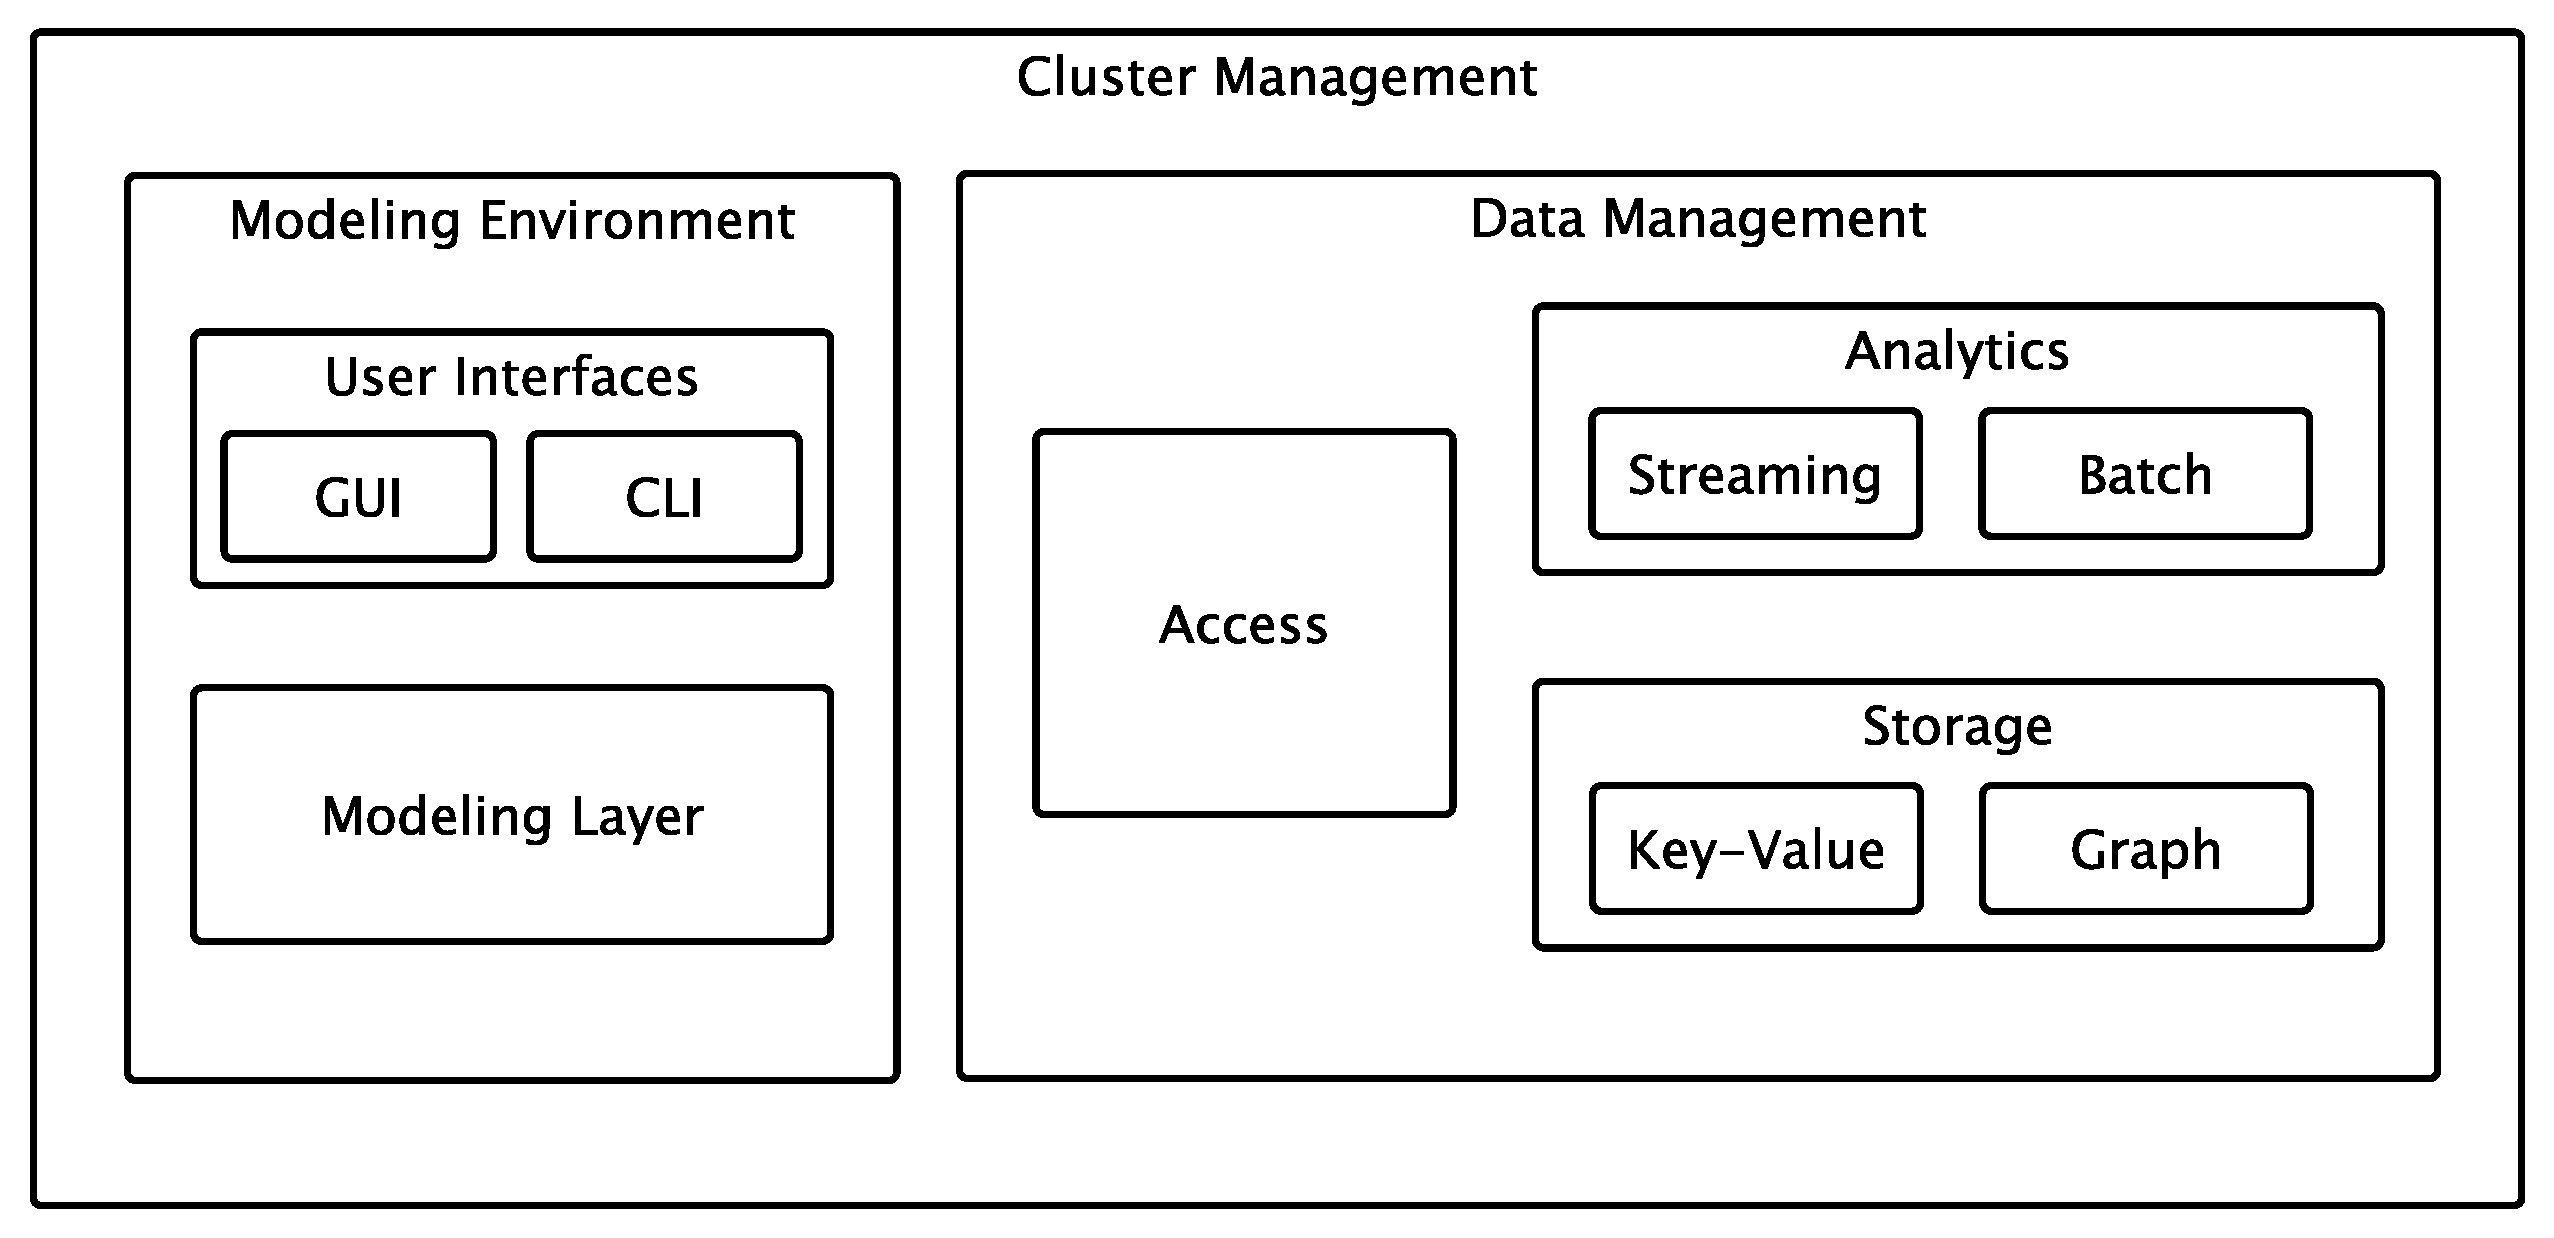
\includegraphics[width=12cm]{img/coarse-grain-schema.pdf}
\caption{High-level architecture design for ScalABM.}
\end{figure}

\subsubsection{Cluster management} 
Current approaches to running large-scale ABMs leverage either...
\begin{itemize}
    \item University/national super-computers: Use FLAME or Repast to build large-scale, complicated models. Both FLAME and Repast use some kind of message passing (but NOT ``peer-to-peer'' message passing) under the hood.
    \item GPU computing: Use CUDA, FLAME GPU (or similar) to build large-scale, simple models.
\end{itemize}
Our strategy for running ABMs at scale will instead leverage massively multi-core cloud computing clusters that are quickly becoming the dominant form of large-scale computing outside of academia.

Benefits to our approach:
\begin{itemize}
    \item Outsourcing of cluster management to third party provider. ABMs built using our framework can be ``containerized'' and sent off to a third-party cloud computing service provider such as \href{http://aws.amazon.com/}{AWS}, \href{https://cloud.google.com/compute/}{Google Compute Engine}, \href{https://www.heroku.com/}{Heroku}, \href{https://mesosphere.com/}{Mesosphere}, etc. This third party provider then handles all of the intricacies involved with scaling up the model on the cluster to meet our needs.
    \item No longer dependent on access to university/national super-computers enhances the reproducibility or our research.  The ability to ``containerize'' an ABM built using out framework means that researchers not directly involved in developing a model can still access all material necessary to completely reproduce that model's output. The container can be used to run the model locally on a laptop or sent to a third party provider to scale up via the cloud. 
\end{itemize}

\subsubsection{Modeling environment}
The modeling environment consists of user interfaces and the modeling layer. The ``front end'' of our modeling environment should consist of two, complementary user interfaces.
\begin{enumerate}
    \item A user-friendly, web-browser based graphical user interface (GUI). The GUI should facilitate interactive exploration of an existing model in near real-time.  The GUI should support real-time data streaming, analysis, and visualization.
    \item An intuitive and consistent command line interface (CLI). In addition to facilitating efficient batch processing of model simulations (i.e., parameter sweeps), the CLI should allow for easy replication of any particular model simulation.
\end{enumerate}

The ``back end'' of our modeling environment is the modeling layer which consists of the actual source code libraries used to implement our ABMs. Important characteristics of our modeling layer:  

\begin{itemize}
    \item The modeling layer should facilitate the construction of new ABMs out of pre-existing, modular components. Novel model components should be able to easily extend pre-existing components. 
    \item Model configuration, including specification of all model parameters as well as the ``wiring'' of model components, should be specified in configuration files that are separate from the actual source code.
\end{itemize}

The modeling layer itself is organized into a number of sub-layers: a behavioral layer, an information layer, and a data analytics layer. See figure \ref{img-figure-2}.
\begin{figure}[H]\label{img-figure-2}
\centering
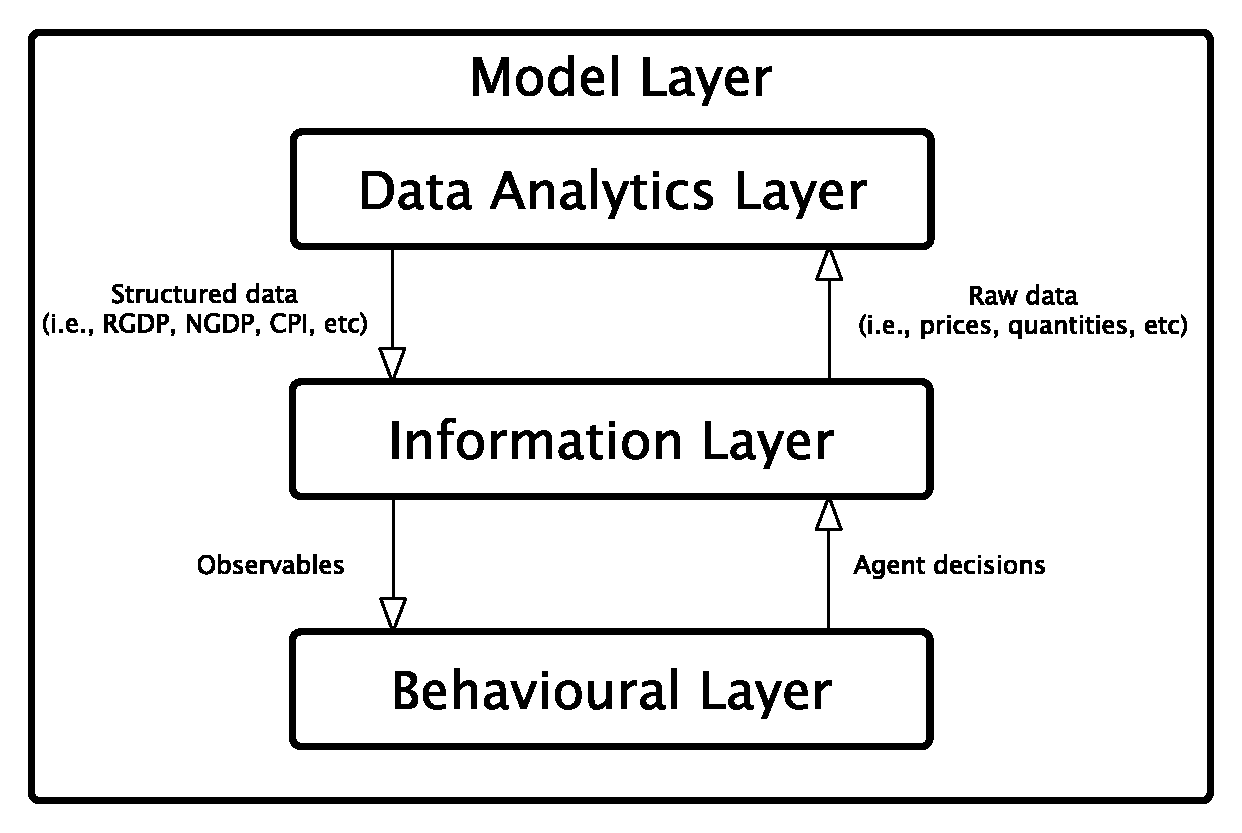
\includegraphics[width=10cm]{img/coarse-grain-model-layer.pdf}
\caption{High-level organization of the modeling layer.}
\end{figure}

\paragraph{Behavioral layer}
An economy is populated with many seemingly disparate types of agents (i.e., consumers, producers, financiers, government, etc).  Our goal with the behavioral layer is to distill the core essence (in terms of data and behaviors) of these different agents into a multi-layered API defining a generic \textit{economic agent} that can then be specialized to the various types of economic agents needed for any particular model.

Several key features distinguish \textit{economic} agents from more generic types of agents. At a minimum these features include: purpose driven (or goal oriented) behaviour, an ability to learn, and the ability to anticipate future events. This suggests that our behavioral layer will need APIs for...
\begin{itemize}
    \item Goals or objectives (and their associated behavioral rules): Our goals/objectives API needs to be as un-opinionated as possible as prospective users of ScalABM are likely to have strong opinions on how to define appropriate goals and decision rules for their agents. At the same time, we will need to have some type of underlying null model of agent goals/objectives. Utility maximization, Belief-Desire-Intent (BDI), probabilistic discrete choice (AKA, random utility maximization) are possibilities.
    \item Learning rules: A large number of various learning rules/mechanisms have been proposed in the academic literature. Roughly, learning rules seem to fall into two camps: learning through previous experience (i.e., reinforcement learning) and learning through observation (i.e., belief learning). Useful references for learning rules for ABMs are the two handbook chapters \href{http://web.uvic.ca/~mingkang/econ353/project/Brenner.pdf}{Brenner (2006)} and \href{http://www.socsci.uci.edu/~duffy/papers/duffy2006.pdf}{Duffy (2006)}.
    \item Expectations formation rules: A large number of various expectation formation rules have been proposed in the literature. Useful references for expectation formation rules are \href{http://feb.kuleuven.be/fac/Slides_Degrauwe/HomHBchapter23.pdf}{Hommes (2006)}, \href{http://econ.columbia.edu/files/econ/content/hommes_background_material_2.pdf}{Anufriev and Hommes (2012)}, \href{http://www.columbia.edu/~mw2230/AREcon.pdf}{Woodford (2013)}, \href{http://www.emeraldinsight.com/doi/pdfplus/10.1108/S0193-230620140000017002}{Assenza et al (2014)}.
\end{itemize}

High-level description of an agent in our framework is a layered collection of behaviors and decision rules...
\begin{figure}[H]
\centering
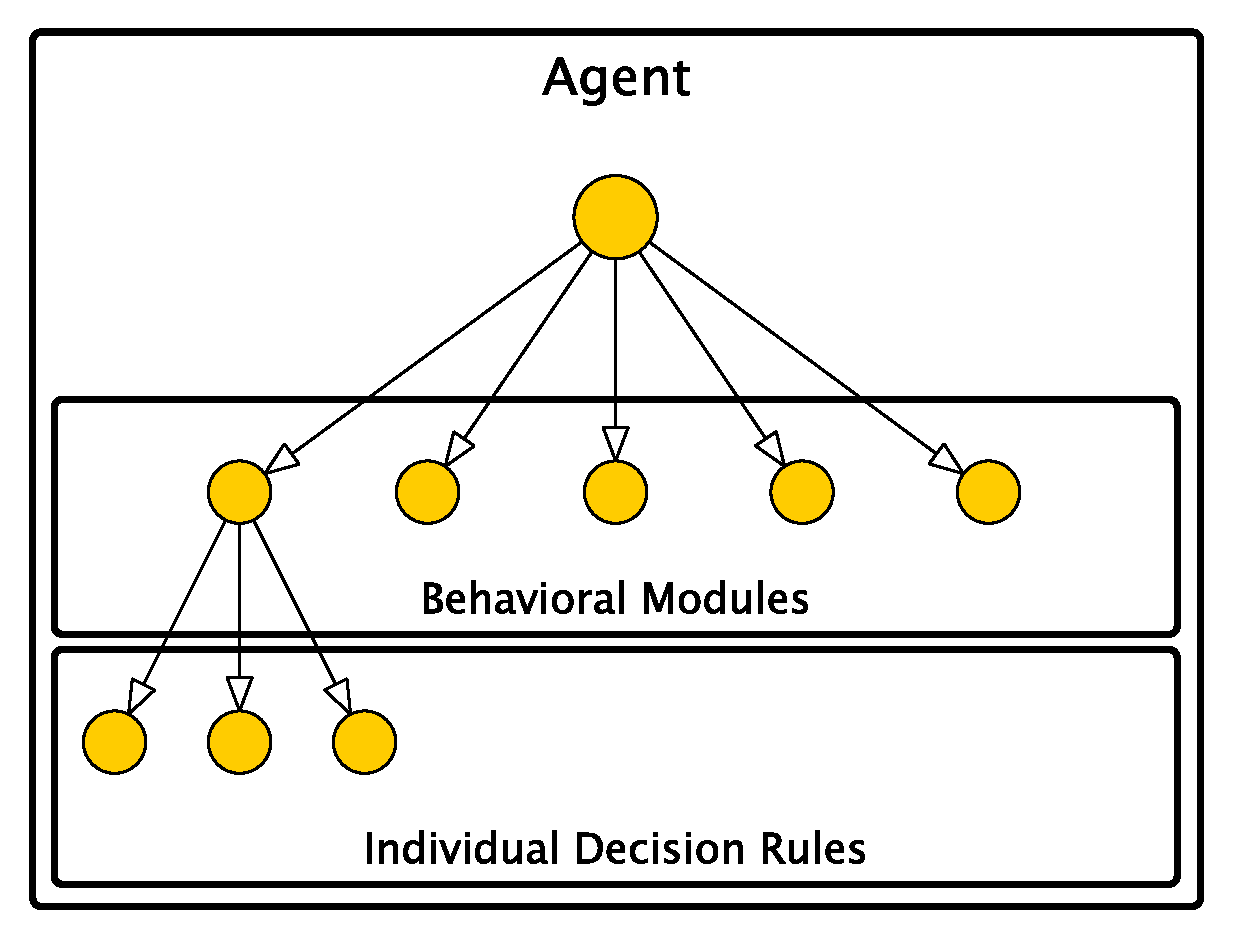
\includegraphics[width=10cm]{img/hierarchical-actor.pdf}
\caption{An agent in our framework is a layered collection of behaviors and decision rules.}
\end{figure}

Concurrent communication between real-world economic agents is a fundamental fact of economic life. Inter-agent communication can be either direct (i.e., ``peer-to-peer'') or indirect (i.e., via market institutions). In order to model both direct and indirect communication between agents in our framework we leverage the \href{https://en.wikipedia.org/wiki/Actor_model}{Actor model} of concurrency. The Actor model treats ``actors'' as the universal primitives of concurrent computation: in response to a message that it receives, an actor can make local decisions (given its information set), possible create more actors, send more messages, determine how to respond to the next message received, etc.

Stock flow consistency is an important property of large-scale macro models, but is not a property that makes sense to impose in general for our framework.  Need to have a behavioral module that implements stock flow consistent accounting rules.

Our economic agents will need to condition their decisions on an information set.  In contrast to (most) DSGE models, information sets in our framework will be highly heterogeneous. The information set for any particular economic agent should consist of three components:
\begin{itemize}
    \item Private information: information that is idiosyncratic to a particular agent. 
    \item Public information: information that a particular agent shares with one or more agents.
    \item Global information: information that is shared between all agents.
\end{itemize}

\begin{figure}[H]
\centering
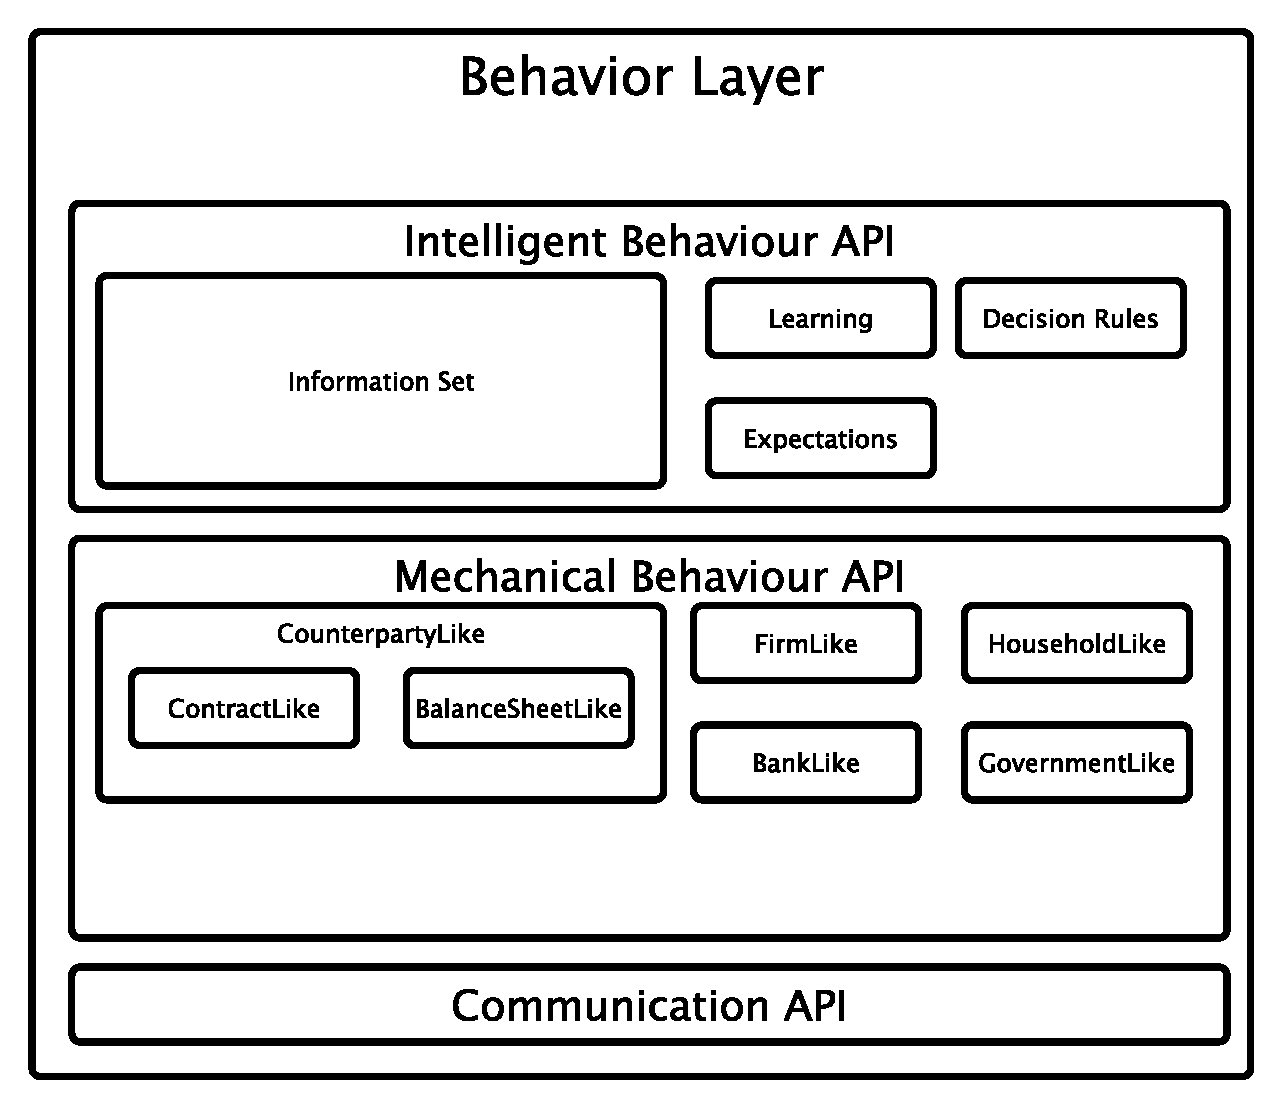
\includegraphics[width=10cm]{img/behavior-layer.pdf}
\caption{???}
\end{figure}


\paragraph{Information Layer}
Markets are institutions that aggregate data: markets take agent decisions/choices as raw data which they aggregate into prices and quantities. These prices and quantities are, typically, but not always observable by others.  Most market prices are public information.
\begin{figure}[H]
\centering
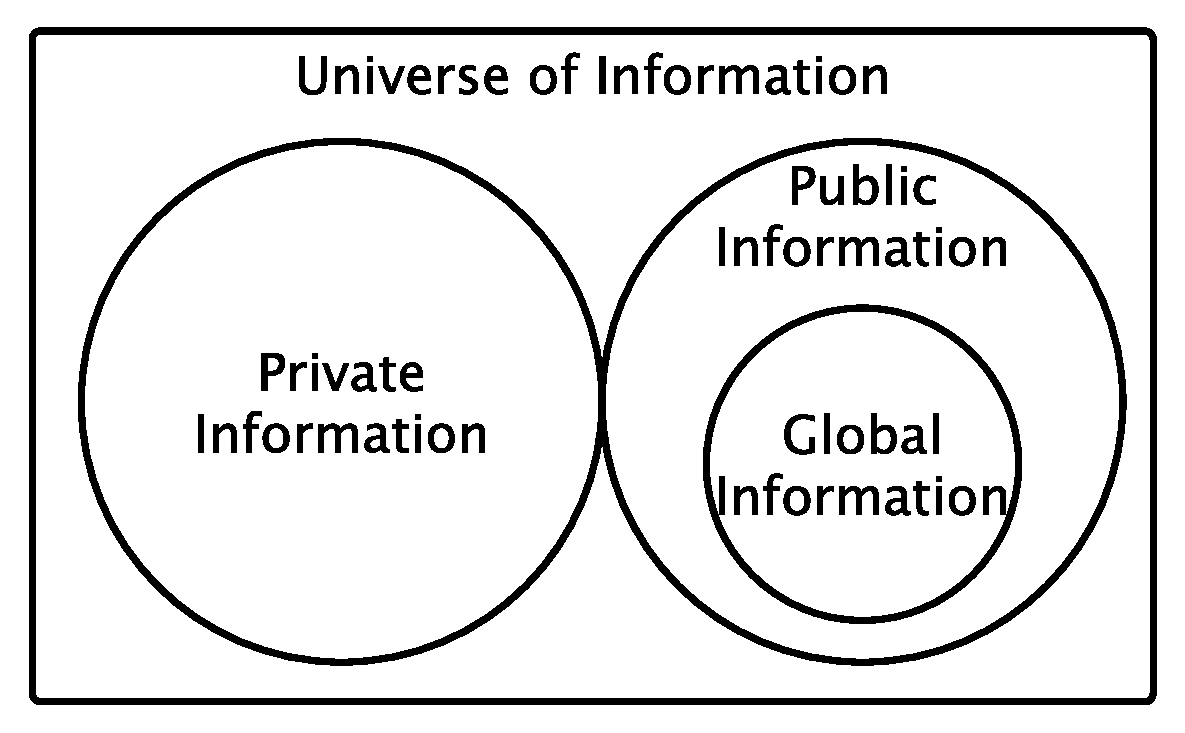
\includegraphics[width=10cm]{img/information-sets.pdf}
\caption{Information set for a particular economic agent.}
\end{figure}

\begin{figure}[H]
\centering
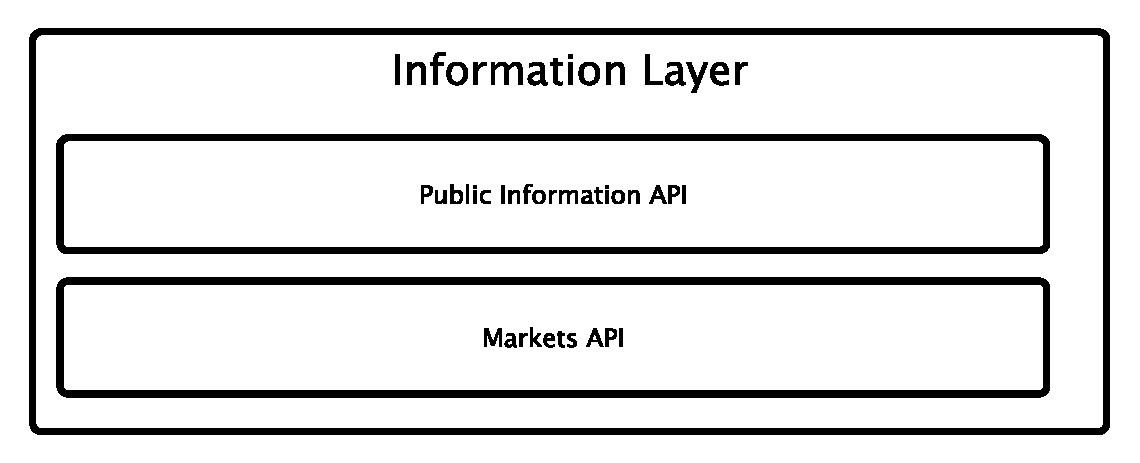
\includegraphics[width=10cm]{img/information-layer.pdf}
\caption{Information layer consists of the markets API and a public information API.}
\end{figure}

\paragraph{Data Analytics Layer}
The data analytics layer encapsulates the functionality for aggregating raw data into additional structured data that agents can use for making decisions.  Specifically, the data analytics layer would contain classes and methods for computing standard macro economic indicators (i.e., real and nominal GDP, stock market index, house price index, consumer price index, unemployment rates, etc). Users should be able to extend the data analytics capabilities as needed for a particular model.


\subsubsection{Data Management}
In order for our ABMs to be data-driven, we need to think carefully about how our framework we will manage the flow and storage of data (both model generated data as well as real-world data). There are (at least!) three components to data management: access, analytics, and storage.
\begin{itemize}
    \item Access: A running ABM will generate a large volume of data. Model generated data might be stored, sent to a data analytics engine, or logged out to a file(s). Additionally, data will likely flow in the reverse direction.  In particular, agents in a running ABM may need to read data from a data store (for example, we might wish to initialize economic agents using real-world data).
    \item Analytics: A running ABM is a continuous source of data whose volume is not predetermined. Put another way: ABMs generate \href{http://www.reactive-streams.org/}{reactive data streams}.  Our data analytics components should therefore include tooling for processing and analyzing streaming data. In addition to processing and analyzing streaming data, we will also need to preform various ``batch'' or ``mini-batch'' computations. Such batch processing jobs would be performed either relatively infrequently on streaming data or upon completion of a model simulation. Our data analytics should include tooling for dealing with batch computations.
    \item Storage: The modeling layer should have read/write access to a scalable data store. Additionally, the data analytics components will need a source of input data. In order to avoid simulations being I/O bound, our data store should have extremely fast write access.
\end{itemize}

\section{Implementation}

\subsection{Platform architecture}

\begin{figure}[H]
\centering
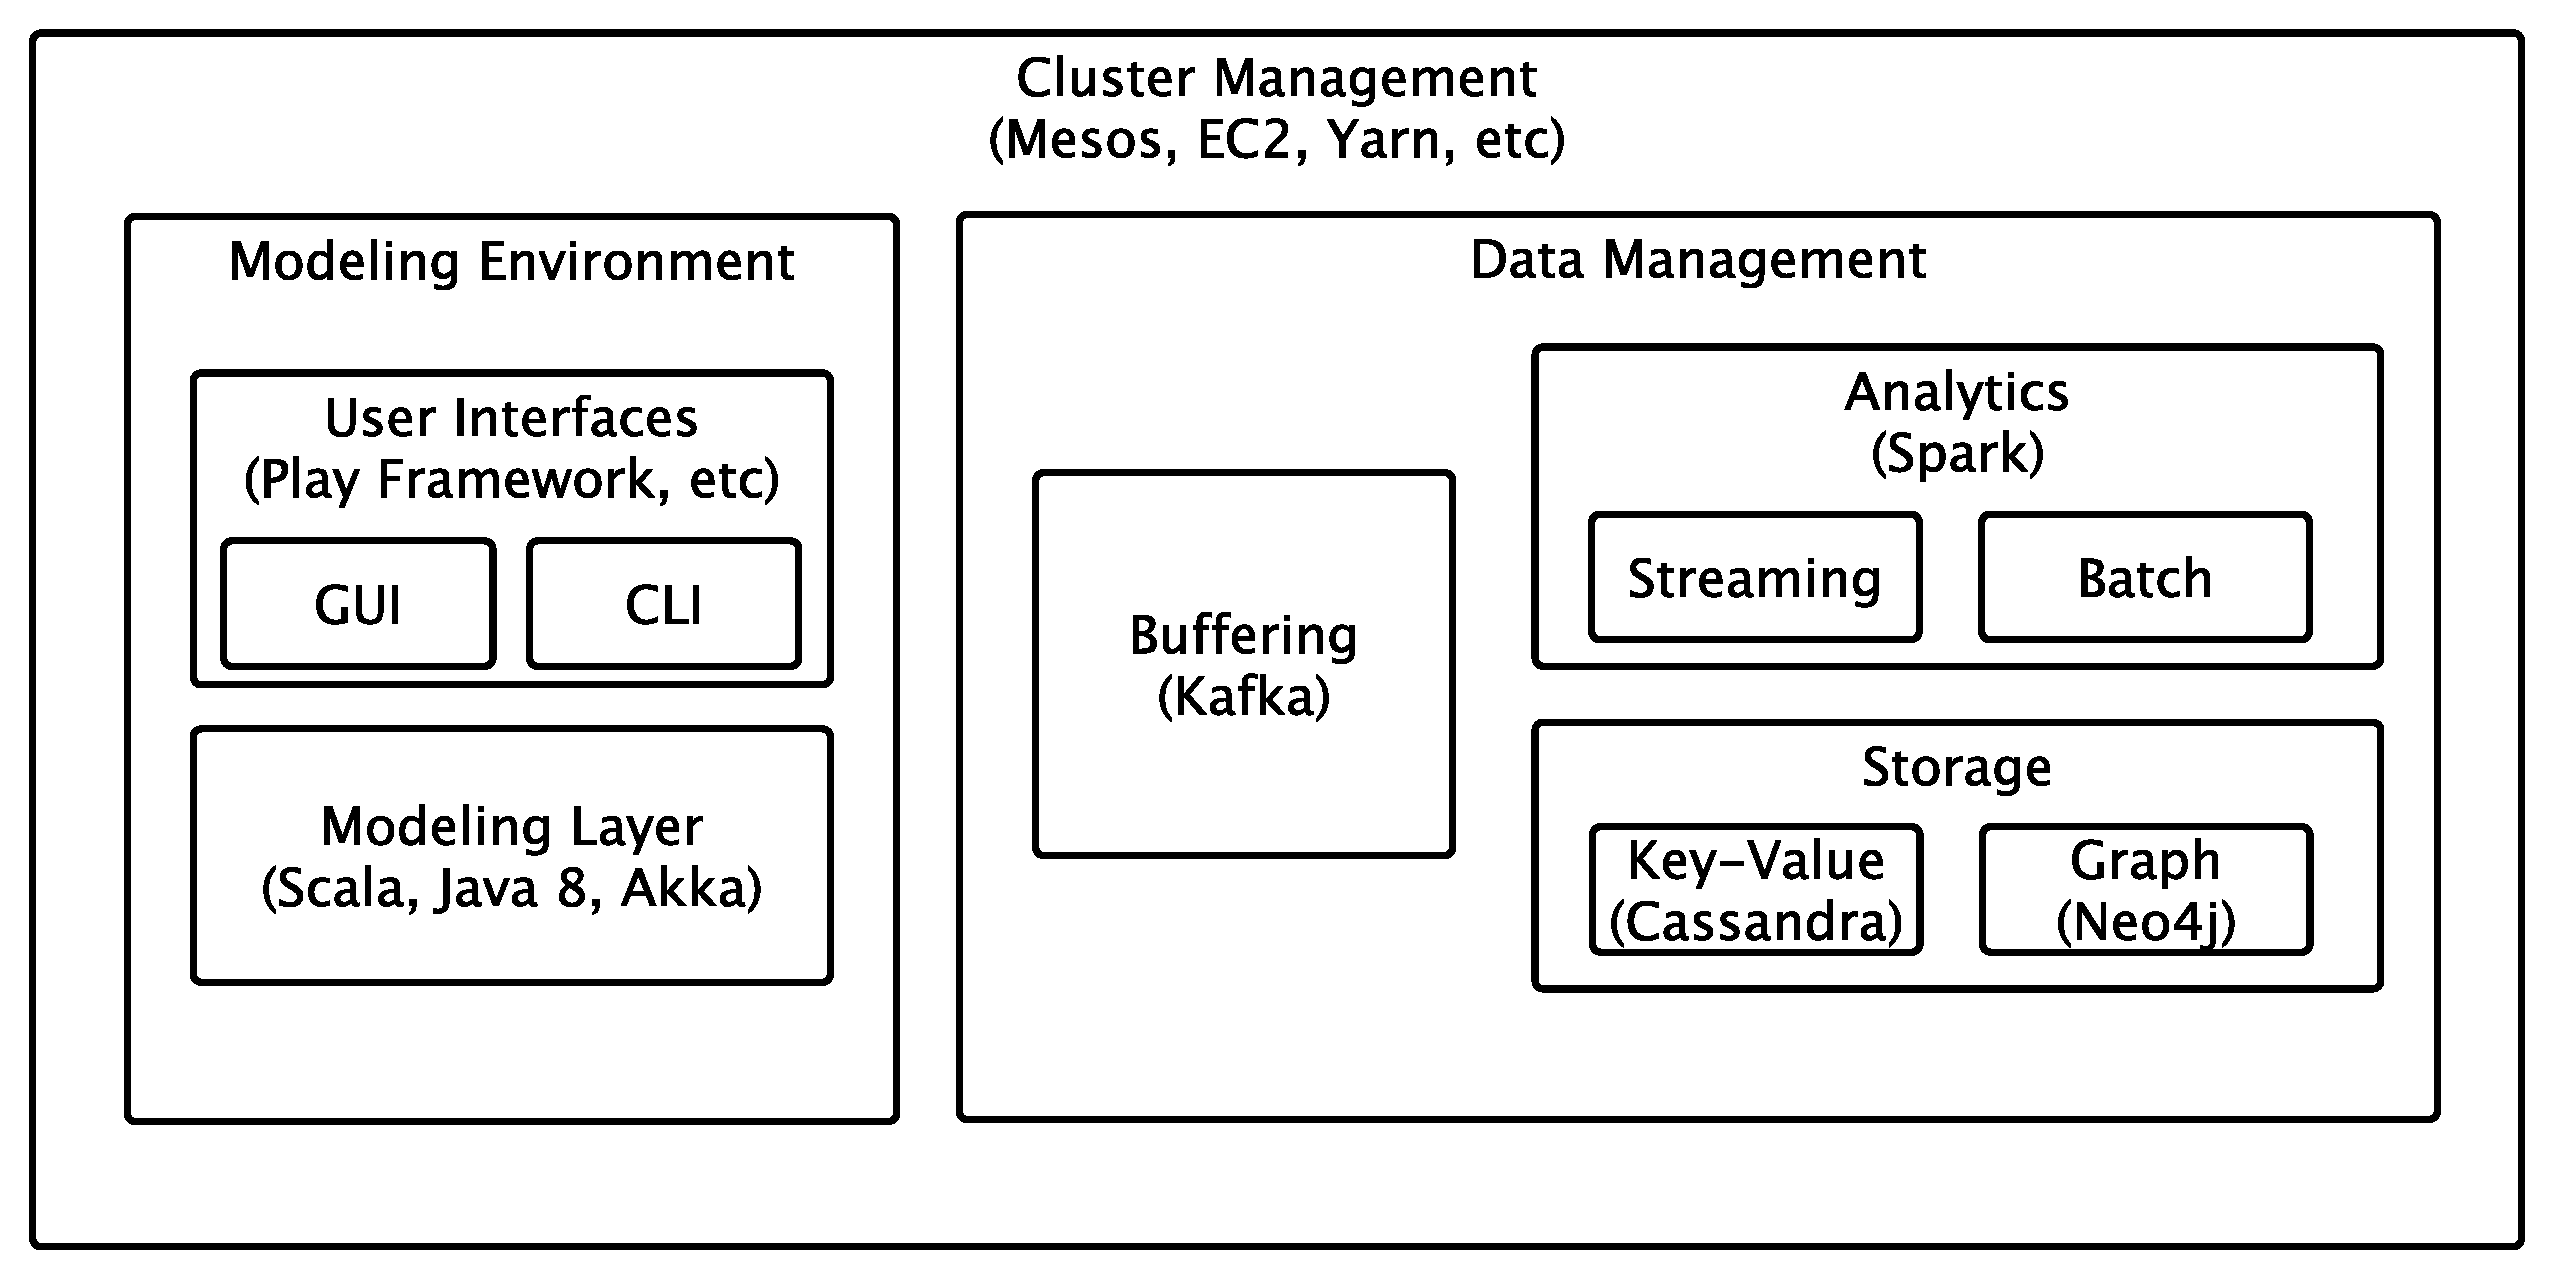
\includegraphics[width=10cm]{img/coarse-grain-schema-2.pdf}
\caption{Macro-grain architecture for ScalABM. }
\end{figure}

\subsubsection{Modeling environment}
Browser based GUI interfaces should be built using the \href{https://www.playframework.com/}{Play} web application framework. The Play framework cleanly integrates Javascript libraries for real-time data analysis and visualization with backend model libraries.

\subsubsection{Data Management}
Broadly speaking, we will need to store two types of data: real-world data and model generated data. The way in which we store our data should be heavily influenced by the types of questions we intend to ask of our data. 
There are two kinds of questions that we will want to ask of our model generated data:
\begin{enumerate}
    \item Questions about cross-sectional and time series properties of model generated data. For these types of questions NoSQL Key-Value databases, such as \href{http://cassandra.apache.org/}{Cassandra},  are ideal data stores. Key-Value databases are designed for storing data in a schema-less way. In a key-value store, each datum consists of an indexed key and a value, hence the name. 
    \item Questions about the network structures between model agents. For questions about network structure, graph databases are ideal.  Graph databases, such as Neo4j, are designed for data whose relations are well represented as a graph and has elements which are interconnected, with an undetermined number of relations between them.
\end{enumerate} 


\subsection{Modeling Layer}
ScalABM leverages the \href{https://en.wikipedia.org/wiki/Actor_model}{Actor model} of concurrency as implemented in the \href{http://akka.io/}{Akka} library to model both direct and indirect communication between economic agents using concurrent, asynchronous message passing.\footnote{
%
Akka is a toolkit and runtime for building highly concurrent, distributed, and resilient message-driven applications on the JVM.
%
} All agents in ScalaABM are implemented as hierarchical trees of Akka Actors.
\begin{figure}[H]
\centering
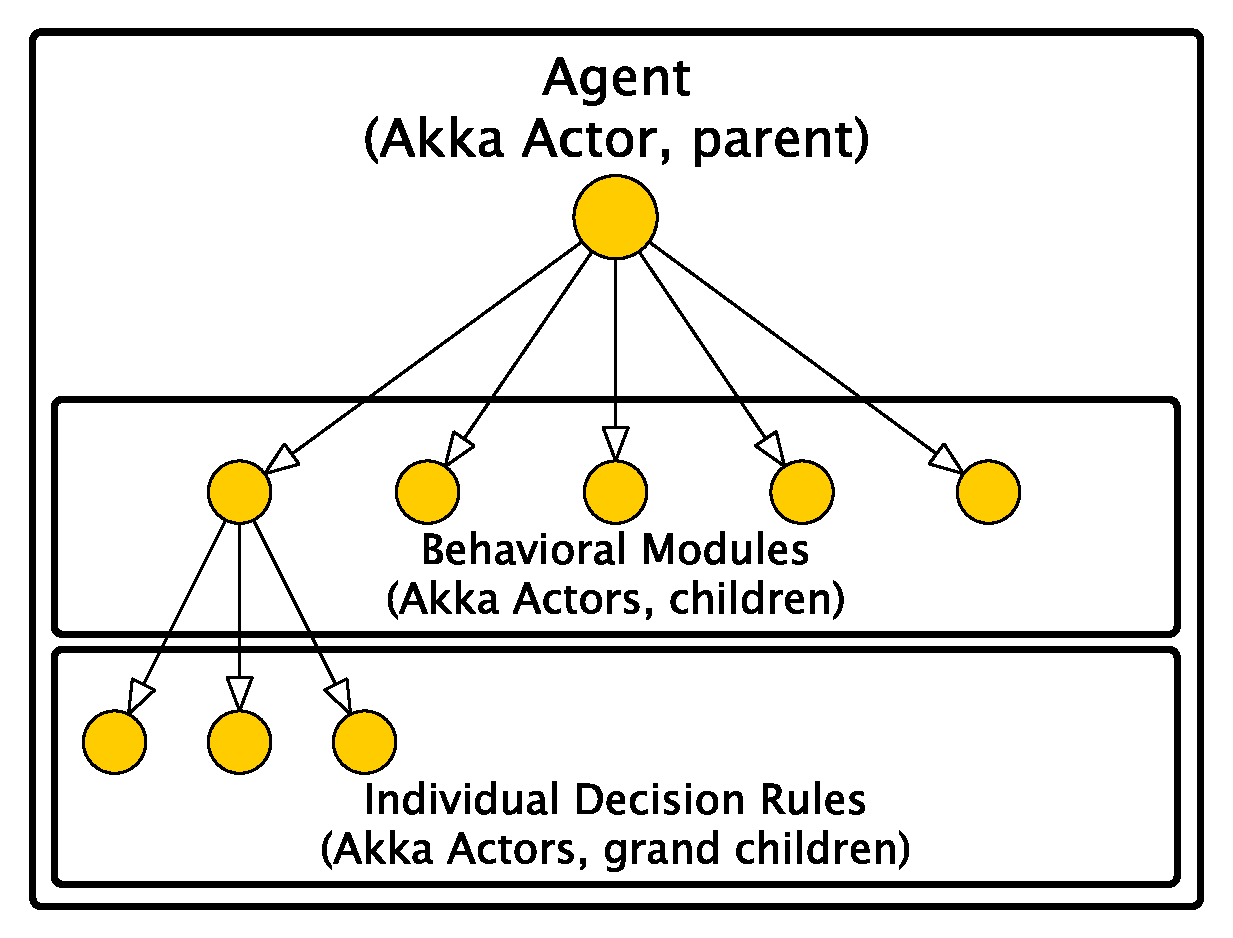
\includegraphics[width=10cm]{img/hierarchical-actor-2.pdf}
\caption{???}
\end{figure}

This design allows an agent to itself be distributed across a cluster efficiently.

\subsubsection{Communication Layer}
In order to impose structure on inter and intra agent communications we have developed an API for a scalable agent communication language for economic agents tentatively called ScalACL. The ScalACL API specifies...
\begin{itemize}
    \item a set of abstract message types that impose structure on the messages passed between a group of economic agents,
    \item a set of abstract protocols that impose structure on conversations (i.e., sequences of messages) between a group of economic agents,
    \item a behavioral trait that allows an agent to communicate using the language.
\end{itemize}
Each abstract message type can be thought of as defining an ``envelope'' containing the actual content of the message that is to be exchanged between a group of economic agents. Defining envelopes containing messages is useful because it allows agents to react based on the type message received. Each abstract protocol defines a particular subset of message types that can be sent by an agent in response to a particular type of message that it has received. 

Our agent communication API is influenced by, but not slave to, the \href{http://www.fipa.org/}{Foundation for Intelligent Physical Agents (FIPA)} compliant \href{http://www.fipa.org/specs/fipa00037/SC00037J.pdf}{Agent Communication Language (ACL)}.

\section{Markets API}

The Markets API explicitly defines various disequilibrium dynamic processes by which market prices and quantities are determined.\footnote{
%
Connection to Sims' ``wilderness of disequilibrium economics'' quote.
%
}

\subsection{Requirements} The Markets API needs to be sufficiently flexible in order to handle markets for relatively homogeneous goods (firm non-labor inputs, firm outputs, final consumption goods, standard financial products etc.) as well as markets for relative heterogeneous goods (i.e., labor, housing, non-standard financial products, etc).

Here is my (likely incomplete) list..
\begin{itemize}
    \item Receive buy and sell orders from other actors.
    \item Accept (reject) only valid (invalid) buy and sell orders.
    \item Handle queuing of accepted buy and sell orders as necessary.
    \item Order execution including price formation and, if necessary, quantity determination.
    \item Processing and settlement of executed orders once those orders have been filled.
    \item Record keeping of orders received, orders executed, transactions processed, etc.
\end{itemize}

Problem: too many requirements for a single market actor to satisfy. Solution: model the market actor as a collection of actors. Specifically, suppose that each MarketLike actor is composed of two additional actors: a ClearingMechanismLike actor that models the clearing process of buy and sell orders, and then a SettlementMechanismLike mechanism that processes the resulting filled orders.

\subsection{MarketLike actor} The MarketLike actor should directly receive buy and sell orders for a particular Tradable, filter out any invalid orders, and then forward along all valid orders to a ClearingMechanismLike actor for further processing.

\subsection{ClearingMechanismLike actor}. A ClearingMechanismLike actor should handle order execution (including price formation and quantity determination as well as any necessary queuing of buy and sell orders), generate filled orders, and send the filled orders to some SettlementMechanismLike actor for further processing. Note that each MarketLike actor should have a unique clearing mechanism.

\subsubsection{Order execution} Order execution entails price formation and quantity determination. Market price formation requires clearing the market. It is important to be clear about the definition of the term ``market clearing'' [?] defines ``market clearing'' as follows:
\begin{enumerate}
    \item The process of moving to a position where the quantity supplied is equal to the quantity demanded.
    \item The assumption that economic forces always ensure the equality of supply and demand.
\end{enumerate}
In most all mainstream macroeconomic models (i.e., RBC, DSGE, etc) it is assumed that economic forces instantaneously adjust to ensure the equality of supply and demand in all markets.\footnote{
%
I am sure that there are important examples in the mainstream economics literature where the process
of market clearing is explicitly modeled and we should cite these.
%
}

In our API, however, a key component of a ClearingMechanismLike actor is a MatchingEngineLike behavioral trait which explicitly defines a dynamic process by which orders are executed, prices are formed, and quantities are determined. Note that a MatchingEngineLike behavioral trait is similar to an auction mechanism in many respects. Friedman (2007) lists four major types of two-sided auction mechanisms commonly implemented in real world markets.\footnote{
%
TODO: similarly classify the various types of single-sided auction mechanisms commonly implemented
in real world markets.
%
}
\begin{itemize}
    \item Posted offer (PO): PO allows one side (say sellers) to commit to particular prices that are publicly posted and then allows the other side to choose quantities. PO is the dominant clearing mechanism used in the modern retail sector.
    \item Bilateral negotiation (BLN): BLN requires each buyer to search for a seller (and vice versa); the pair then tries to negotiate a price and (if unsuccessful) resumes search. BLN clearing mechanisms were prevalent in preindustrial retail trade, and continue to be widely used in modern business-to-business (B2B) contracting. Some retail Internet sites also use BLN clearing mechanisms.
    \item Continuous double auction (CDA): CDA allows traders to make offers to buy and to sell and allows traders to accept offers at any time during a trading period. Variants of CDA markets prevail in modern financial exchanges such as the New York Stock Exchange (NYSE), NASDAQ, and the Chicago Board of Trade and are featured options on many B2B Internet sites.
    \item Call auction (CA): The CA requires participants to make simultaneous offers to buy or sell, and the offers are cleared once each trading period at a uniform price. Each of these auction mechanisms would correspond to a particular implementation of an MatchingEngineLike behavior.
\end{itemize}

\subsubsection{Order queuing} Order queuing involves storing and possibly sorting received buy and sell orders according to some OrderQueuingStrategy. Different order queuing strategies will be distinguished from one another by...
\begin{itemize}
    \item type of mutable collection used for storing buy and sell orders,
    \item the sorting algorithm applied to the mutable collections.
\end{itemize}

For example, some OrderQueuingStrategy behaviors might only require that unfilled buy and sell orders are stored in some mutable collection (the sorting of buy and sell orders within their respective collections being irrelevant). Other OrderQueuingStrategy behaviors might have complicated OrderBookLike rules for sorting the stored buy and sell orders. Here is a quick sketch of what the code for generic OrderQueuingStrategy would look like...

\subsection{Settlement mechanisms} Fundamental objective of a SettlementMechanismLike actor is to convert filled orders into settled transactions. Rough sketch of a process by which filled orders are converted into settled transaction is as follows.
\begin{itemize}
    \item Receive filled orders from some ClearingMechanismLike actor(s).
    \item Send request for the desired quantity of the specified Tradable to the seller. 
    \item Send request for some desired quantity of the specified means of payment (which will be some other Tradable) to the buyer.
    \item Handle response from the seller (requires handling the case in which seller has insufficient quantity of the specified Tradable).
    \item Handle response from the buyer (requires handling the case in which buyer has insufficient quantity of the specified means of payment).
    \item Generate a settled transaction.
\end{itemize}

The following two types of settlement mechanisms should cover most all possible use cases.
\begin{itemize}
    \item Bilateral settlement: with bilateral settlement, buy and sell counterparties settle directly with one another.
    \item Central counterparty (CCP) settlement: With CCP settlement, a central counterparty (CCP) actor inserts itself as a both a buy and sell counterparty to all filled orders that it receives from some clearing mechanism. After inserting itself as a counterparty, the CCP actor then settles the filled orders using bilaterally. Unlike clearing mechanisms, which are unique to a particular market, settlement mechanisms could be shared across markets.
\end{itemize}

\section{Use cases for MarketLike actors}

\subsection{Specific use cases for MarketLike actors} In this section I sketch out some specific use cases for the Markets API.

\subsubsection{Retail goods market}. RetailMarketLike behavior would extend MarketLike behavior with:
\begin{itemize}
    \item Clearing mechanism with PostedOfferLike matching engine,
    \item BilateralSettlement settlement mechanism.
\end{itemize}
Retail goods markets are markets for final consumption goods (typically purchased by households).

\subsubsection{Wholesale goods market} WholesaleMarketLike behavior would extend MarketLike behavior with:
\begin{itemize}
    \item Clearing mechanism with BilateralNegotiationLike matching engine,
    \item BilateralSettlement settlement mechanism.
\end{itemize}
Wholesale goods markets are markets for intermediate goods (typically purchased by firms and then used in the production of retail goods).

\subsubsection{Labor market} LaborMarketLike behavior would extend MarketLike behavior with:
\begin{itemize}
    \item Clearing mechanism with either BilateralNegotiationLike or PostedOffer matching engines,
    \item BilateralSettlement settlement mechanism.
\end{itemize}
Labor markets are tricky. If we use BilateralNegotiationLike clearing mechanism then we can link into the massive search and match literature.

\subsubsection{Housing market} HousingMarketLike behavior would extend MarketLike behavior with:
\begin{itemize}
    \item Clearing mechanism with PostedOfferLike matching engine,
    \item BilateralSettlement settlement mechanism.
\end{itemize}
Note similarity of HousingMarketLike to RetailMarketLike

\subsubsection{Securities market}. SecuritiesMarketLike behavior would extend MarketLike behavior with:
\begin{itemize}
    \item Clearing mechanism with ContinuousDoubleAuctionLike matching engine and OrderBookLike order queuing strategy,
    \item CentralCounterpartySettlement settlement mechanism.
\end{itemize}
Securities markets would include markets for stocks, bonds, and currencies. Could even create a SecuritiesExchange actor which would route orders for various securities to the appropriate SecuritiesMarketLike actor.

\subsubsection{Unsecured interbank lending market} InterbankMarketLike behavior would extend MarketLike behavior with:
\begin{itemize}
    \item Clearing mechanism with BilateralNegotiationLike matching engine,
    \item BilateralSettlement settlement mechanism.
\end{itemize}
See Perry Mehrling for more details on unsecured interbank lending markets.

\subsubsection{Secured interbank lending (repo) market} RepoMarketLike behavior would extend MarketLike behavior with:
\begin{itemize}
    \item Clearing mechanism with BilateralNegotiationLike matching engine,
    \item BilateralSettlement settlement mechanism.
\end{itemize}
See Perry Mehrling for more details on secured interbank lending (repo) markets.

% \section{Economics as distributed computation}
% Major source of motivation for our approach is Rob Axtell's \href{http://www.researchgate.net/profile/Robert_Axtell2/publication/228586815_Economics_as_distributed_computation/links/0a85e536b81c27f06e000000.pdf}{2002 Brookings working paper}.

% \subsection{Concurrency vs parallelism}
% Discuss the difference between parallelism and concurrency. See this \href{http://stackoverflow.com/questions/1050222/concurrency-vs-parallelism-what-is-the-difference}{SO} post for details. Concurrency is a more general type of parallelism. Economic systems are concurrent.

% \subsection{Asynchronous vs synchronous}
% Discuss the difference between synchronous and asynchronous execution. Economic systems are asynchronous not synchronous.

% \subsection{Economics is concurrent, asynchronous distributed computing}
% Concurrent, asynchronous In his , Rob discusses have noted that the economy is a distributed system which provides a motivation for our use of Scala and Akka to implement our framework (both were developed specifically for building scalable distributed systems). Contrast with other ABM frameworks, programming lanaguages, etc.

%There is a sense in which economics can be reduced to a combination of accounting and agent decision making.  

\end{document}
